Chapter \ref{chap:msre} verified the hybrid $S_N$-diffusion method implemented in Moltres through
1-D, 2-D, and 3-D
$k$-eigenvalue simulations of the \gls{MSRE} against the OpenMC Monte Carlo neutron transport code
for molten salt reactor control rod modeling. The 3-D simulations validated the 3-D \gls{MSRE}
model in this work against \gls{MSRE} experimental data and the \gls{MSRE} numerical benchmark
study \cite{fratoni_molten_2020} in the context of the initial criticality and rod worth
measurement experiments. The 3-D simulations also showed that the hybrid method runs with
reasonable computational costs compared to the standard neutron diffusion method and exhibited
efficient strong scaling across compute nodes.

This chapter builds on the foundations of Chapter \ref{chap:msre} to validate the hybrid
method for neutronics modeling in time-dependent 3-D simulations of reactivity-initiated
transients. This chapter presents simulation results from Moltres for the \gls{MSRE} rod drop
experiment. Beyond time-dependent modeling with the hybrid method, the simulations will also
demonstrate compatibility between the existing neutronics/thermal-hydraulics coupling
capabilities in Moltres and the newly-implemented hybrid method.

Section \ref{sec:rod-drop} covers the model setup, numerical results, and discussion of the rod
drop experiment.
%Section \ref{sec:reactivity-insertion} covers the model setup, numerical results,
%and discussion of the reactivity insertion experiment.
Section \ref{sec:transient-summary}
summarizes the findings from the rod drop experiment study.

\section{Rod Drop Experiment} \label{sec:rod-drop}

\gls{MSRE} researchers conducted a series of rod drop experiments at three different $^{235}$U
loadings \cite{prince_zero-power_1968}. These experiments were conducted from an initially critical
and low power state with an initial neutron count rate of approximately 30,000 counts per second
from neutron detectors placed near the reactor. A rapid-action camera photographed the integral
count shown on the detectors about once every second starting from a few seconds before the rod
drop to about thirty seconds after the rod drop.

This work aims to replicate the integral count curve following a rod drop of Rod 1 with the
$^{235}$U loading corresponding to ``30 capsule additions'' of highly-enriched $^{235}$U capsules
into the \gls{MSRE} through the ``pump bowl''. Each capsule contains 85 g of $^{235}$U, of which
94.94 \% enters the core
due to residual fuel salt remaining in the drain tanks after mixing \cite{fratoni_molten_2020}.

\subsection{Model Setup} \label{sec:rod-drop-setup}

The key experimental parameters to simulate the rod drop experiment are: the exact $^{235}$U
loading, the initial and final rod heights, the total reactivity withdrawn, and the speed of the
rod drop.

The \gls{MSRE} achieved initial criticality after eight capsule additions with Rod 1 inserted to a
height of 46.6 inches relative to the fully inserted height \cite{prince_zero-power_1968}.
From the \gls{MSRE} experimental rod worth
data, the rod worth evaluates to approximately 72 pcm relative to the fully withdrawn state; the
$k_\text{eff}$ of the \gls{MSRE} at initial criticality with Rod 1 fully withdrawn would be
1.00072. According to the same \gls{MSRE} report, the
authors back-calculated the critical $^{235}$U loading with Rod 1 fully withdrawn to be 65.25 kg.
They also provided a $^{235}$U concentration reactivity coefficient of 0.223 $(\delta k/k)/(\delta m
/m)$, where $k$ is the multiplication factor and $m$ is the $^{235}$U mass. The excess $^{235}$U
mass at initial criticality compensating for Rod 1 inserted to 46.6
inches can estimated through the following steps:
%
\begin{align}
  \frac{\Delta k / k}{\Delta m / m} &= 0.223 \nonumber \\
  \frac{m}{k}\frac{dk}{dm} &= 0.223 \nonumber \\
  \int^{1.00072}_1 \frac{1}{k}\ dk &= 0.223 \int^{65.25+\Delta m}_{65.25} \frac{1}{m}\ dm \nonumber \\
  \ln \left(1.00072\right) &= 0.223 \ln\left(\frac{65.25+\Delta m}{65.25}\right) \nonumber \\
  \Delta m &= 0.2109 \mbox{ kg}.
\end{align}
%
This change in mass is equivalent to approximately 2.61 highly-enriched $^{235}$U capsules.
Therefore, the $^{235}$U loading for the rod drop experiment is:
%
\begin{gather}
  m_\text{rod drop} = 65.25 \text{kg} + (30 - 8 + 2.61) * 0.085 \text{kg} * 0.9494 = 67.24 \text{kg}
\end{gather}
%
The $k_\text{eff}$ of the \gls{MSRE} with 67.24 kg loading and all rods fully withdrawn is:
%
\begin{align}
  \int^{k_{67.24 \text{kg}}}_1 \frac{1}{k}\ dk &= 0.223 \int^{67.24}_{65.25} \frac{1}{m}\ dm \nonumber \\
    k_{67.24 \text{kg}} &= 1.00671
\end{align}

\begin{figure}[h]
  \centering
  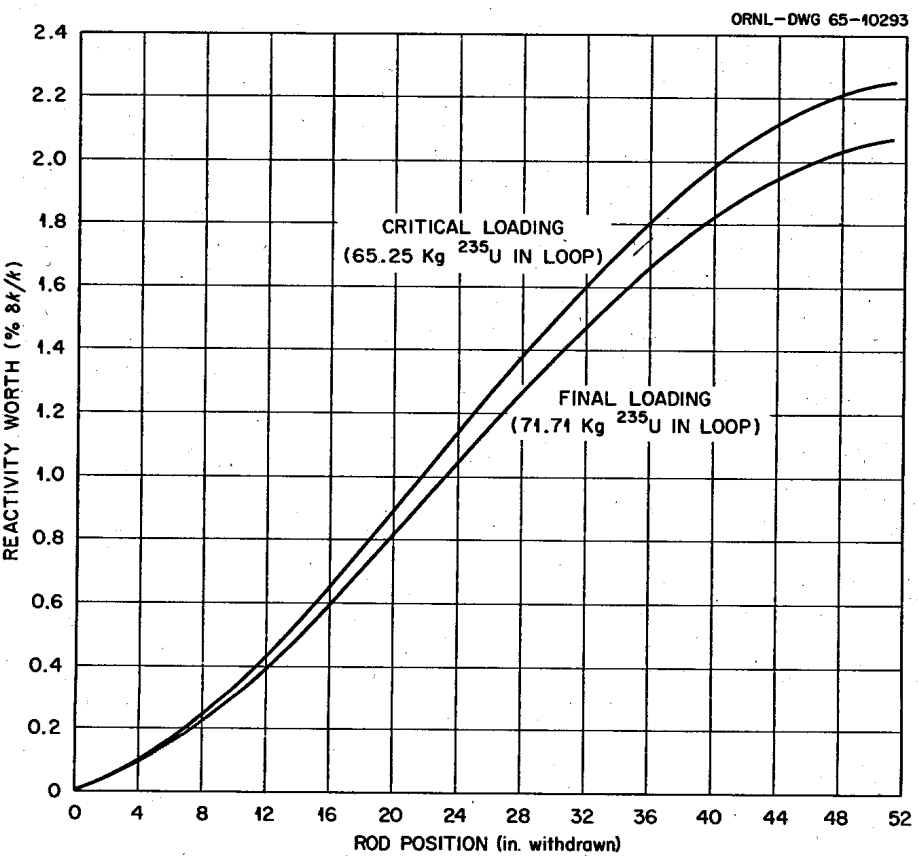
\includegraphics[width=0.6\columnwidth]{msre-rod-worth}
  \caption{Integral control rod worth of Rod 1 \cite{prince_zero-power_1968} at critical and final
  $^{235}$U loading. The final loading rod worth curve is scaled down by 1.087 relative to the
  critical loading rod worth curve.}
  \label{fig:msre-rod-worth-2}
\end{figure}

When loading more $^{235}$U into the core, the shape of the integral rod worth does not change,
but the magnitude scales down by a factor of 1.087 between the critical and final loading
as shown in Figure \ref{fig:msre-rod-worth-2}. After applying this scaling factor to the monotone cubic
spline interpolated \gls{MSRE} rod worth curve, the initial height of Rod 1 to keep the \gls{MSRE}
with 67.24 kg loading critical is approximately 30.75 inches. During the rod drop experiment, the rod
drops from this height to its fully inserted state at 0 inches. This drop induces a total
reactivity withdrawal of 1500 pcm.

The rod drop simulation uses the hybrid $S_N$-diffusion method in Moltres on the verified 3-D
\gls{MSRE} model from Chapter
\ref{chap:msre} at the critical $^{235}$U loading. Refer to Section \ref{sec:3d-model-setup} for
details on the 3-D model. The initial rod height for the \gls{MSRE} model to induce a similar total
reactivity withdrawal of 1500 pcm from Rod 1 drop is 29.4 inches. The acceleration of the
rod is approximately 15 ft s$^{-2}$ from prior testing \cite{prince_zero-power_1968}. At this
acceleration, the rod reaches its fully inserted height at $t=0.4046$ s. Figure \ref{fig:rod-height}
shows the evolution of rod height at each timestep within the first second of the rod drop simulation.

\begin{figure}[htb!]
  \centering
  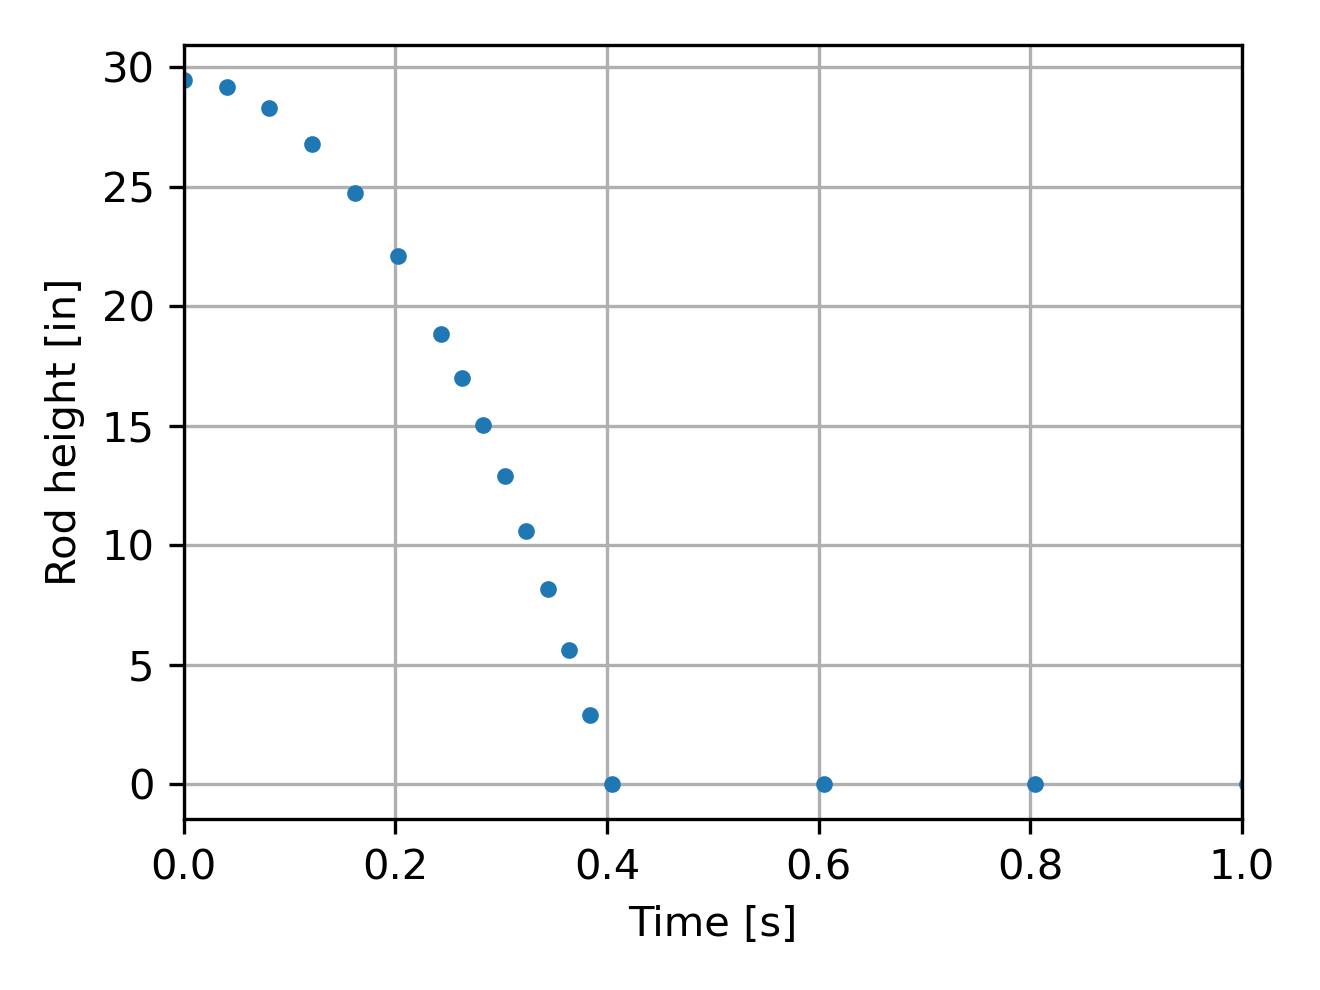
\includegraphics[width=0.7\columnwidth]{rod-height}
  \caption{Evolution of rod height evaluated at each timestep within the first second of the rod
  drop simulation. The rod reaches its fully inserted height at $t=0.4046$ s.}
  \label{fig:rod-height}
\end{figure}

A significant change for the rod drop simulation compared to the $k$-eigenvalue 3-D simulation,
other than the time-dependence, is the inclusion of \glspl{DNP} for the delayed neutron response.
I used the \gls{MOOSE} MultiApp capability available in Moltres to set up a nested iterative
coupling structure for the hybrid
$S_N$-diffusion method with \glspl{DNP} such that the neutron diffusion and \gls{DNP} solvers are
coupled through inner iterations and the $S_N$ solver is coupled them through outer iterations.
Figure \ref{fig:rod-drop-coupling} illustrates this iterative coupling structure and the data
transfers between the solvers. The \gls{DNP} solver is a preexisting capability in Moltres
described in Section \ref{sec:moltres-physics}. For the rod drop simulation, the salt velocity and
\gls{DNP} diffusion coefficients were set to zero, i.e., static salt condition. The simulation
grouped the \glspl{DNP} into six \gls{DNP} decay groups automatically determined by the
ENDF/B-VII.1 nuclear data library \cite{chadwick_endf/b-vii.1_2011} and OpenMC during group
constant generation.

\begin{figure}[t]
  \tikzstyle{every node}=[font=\small]
  \centering
  \begin{tikzpicture}
    \node (1) [solver] {\textbf{$\bm{S_N}$ transport subsolver}};
    \node (2) [solver, right of=1, xshift=4cm] {\textbf{Neutron\\ diffusion\\ subsolver}};
    \node (3) [solver, right of=2, xshift=4cm] {\textbf{DNP subsolver}};
    \draw [arrow] (1.10) -- node[anchor=south, text width=4cm, align=center] {$\vec{D}_g, \gamma_g$} (2.170);
    \draw [arrow] (2.190) -- node[anchor=north, text width=4cm, align=center] {$\phi_g, C_i$} (1.350);
    \draw [arrow] (2.10) -- node[anchor=south, text width=4cm, align=center] {$Q_f, Q$} (3.170);
    \draw [arrow] (3.190) -- node[anchor=north, text width=4cm, align=center] {$C_i$} (2.350);
    \node (5) [bound, fit=(2) (3), inner sep=8pt, label={[align=left]above:\textbf{Inner iteration}}] {};
    \node (6) [bound, fit=(1) (5), inner sep=15pt, label={[align=left]above:\textbf{Outer iteration}}] {};
  \end{tikzpicture}
  \caption{The nested iteration structure coupling the $S_N$, neutron diffusion, and \gls{DNP}
  solvers for the rod drop simulation using the hybrid $S_N$-diffusion method.}
  \label{fig:rod-drop-coupling}
\end{figure}

The output of a $k$-eigenvalue simulation with the rod at the prescribed initial height provides
the initial group flux and \gls{DNP} distributions for the rod drop simulation. The time-depedent
rod drop simulation uses the \gls{MOOSE} Restart capability to load the variable distributions from
the prior $k$-eigenvalue simulation. The total fission neutron production rate at every timestep
is normalized to match the 30,000 counts per second at $t=0$ s from the \gls{MSRE} rod drop
experimental measurements.

\subsection{Rod Cusping Effect Correction}

In deterministic codes with spatial discretization, the material interfaces of a partially-inserted
control rod may not always align with mesh elements. This results in a heterogenous
mesh element that is composed of a control rod material at the top and a non-rod material at the
bottom (for control rods that are inserted from above). The rod cusping effect occurs when
homogenizing mixed mesh elements using the volume weighting method to combine dissimilar material
neutron group constants. Rod cusping error typically decreases with increasing axial mesh
resolution because the size of the mixed mesh elements become smaller relative to the entire
problem domain.

Several rod cusping correction methods exist in literature that are variations of the flux-volume
weighting approach to generate more accurate homogenized group constants in the mixed mesh
elements \cite{yamamoto_cell_2004, graham_subplane_2018, schunert_control_2019}. However, due to
a failed flux-volume weighting implementation and time constraints, this work uses an empirical
approach for rod cusping effect correction. The empirical approach involves precomputing the
$k_\text{eff}$ with the control rod at various levels of insertion within a mesh element. These
simulations apply a simple volume weighting approach to compute a homogenized group constant value
as follows:

\begin{figure}[t]
    \centering
    \begin{subfigure}[t]{.49\textwidth}
        \centering
        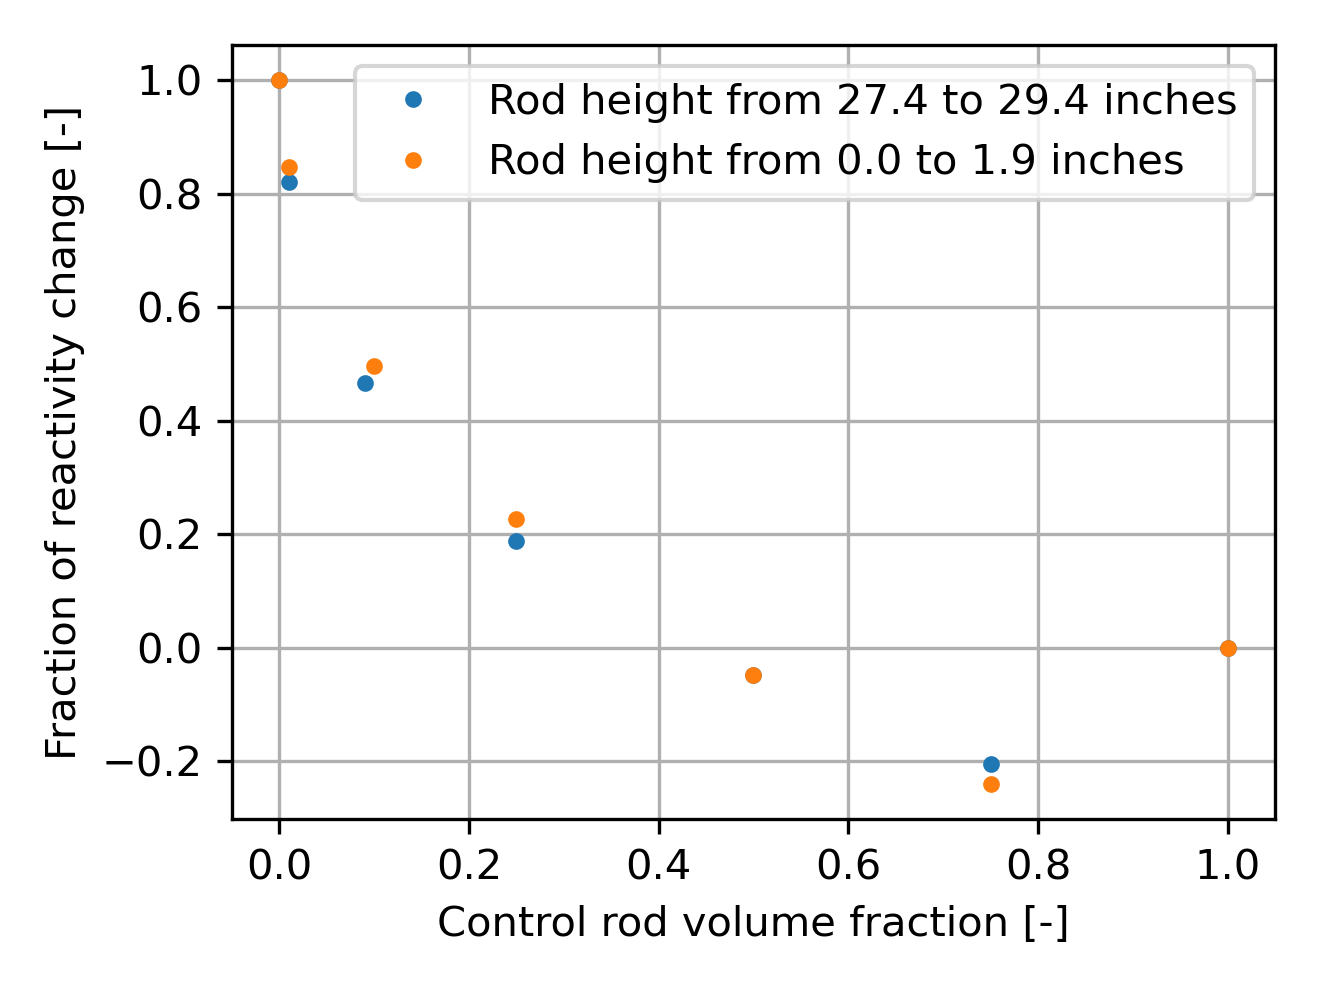
\includegraphics[width=\textwidth]{rod-cusping-1}
        \caption{Uncorrected volume weighting}
        \label{fig:rod-cusping-1}
    \end{subfigure}
    \hfill
    \begin{subfigure}[t]{.49\textwidth}
        \centering
        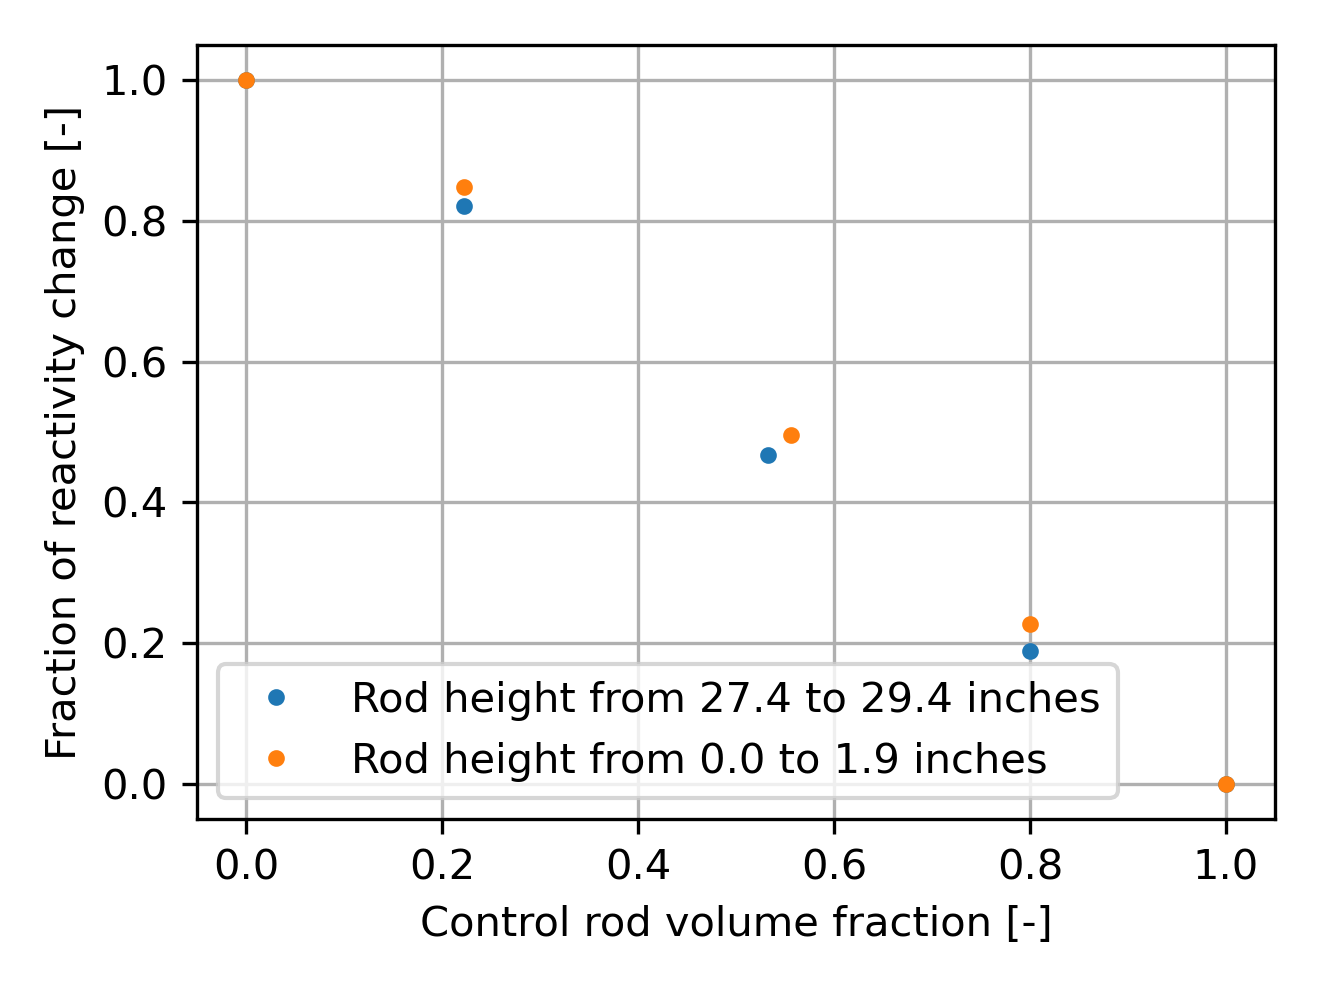
\includegraphics[width=\textwidth]{rod-cusping-2}
        \caption{Corrected volume weighting}
        \label{fig:rod-cusping-2}
    \end{subfigure}
    \caption{Fraction of reactivity change against control rod volume fraction in mixed mesh
    elements with the rod inserted at mid-reactor height (27.4 to 29.4 inches) and full insertion
    height (0.0 to 1.9 inches).}
    \label{fig:rod-cusping}
\end{figure}

\begin{gather}
  \Sigma_\text{vw} = \frac{V_\text{r} \Sigma_\text{r} + V_\text{nr} \Sigma_\text{nr}}{V_\text{r} + V_\text{nr}} \label{eq:vw}
  \shortintertext{where}
  \begin{align*}
    \Sigma_\text{vw} &= \mbox{ volume-weighted group constant in mixed mesh element,} \\
    V_\text{r} &= \mbox{ rod volume fraction in mixed mesh element,} \\
    \Sigma_\text{r} &= \mbox{ rod group constant value,} \\
    V_\text{nr} &= \mbox{ non-rod volume fraction in mixed mesh element,} \\
    \Sigma_\text{nr} &= \mbox{ non-rod group constant value.}
  \end{align*}
\end{gather}

Note that vertical material and mesh interfaces in the 3-D \gls{MSRE} model always align perfectly
because the control rod moves vertically. Therefore, the mixed mesh elements occur only around the
bottom tip of the control rod. Additionally, the volume fraction is equivalent to the height
fraction, and all mixed mesh elements at the same height share the same volume fraction. Figure
\ref{fig:rod-cusping-1} shows how the fraction of reactivity change changes with the control rod
volume fraction when the control rod is at around mid-reactor and full insertion heights. The data
points depict the nonlinear relation between the reactivity change and volume fraction that the
``cusping effect'' is named after. Within this small range of rod motion, the relation should be
approximately linear.

Recognizing that the rod cusping effect approximately follows a $y=x^p$ curve profile, I applied
curve-fitting to obtain the reactivity changes using corrected volume fractions shown in Figure
\ref{fig:rod-cusping-2}. The corrected volume fraction $V_r'$ is calculated as follows
%
\begin{align}
  V_r' &= cV_r^p
  \shortintertext{where}
  p &= 2.5148, \nonumber \\
  c &= 0.43807. \nonumber
  \end{align}
%
The corrected volume fraction produces the desired approximately linear relation between reactivity
change and control rod volume fraction. While this empirical approach worked reasonably well for
this study, a more robust technique will be necessary for future control rod simulations beyond
this work.

\subsection{Rod Drop Numerical Results \& Discussion}

Figure \ref{fig:count-rate} shows the neutron count rate following the rod drop from Moltres. It
shows the steep initial decline in neutron count rate as the rod drops further into the core. The
decline slows at around $t=0.5$ s due to the delayed response of \glspl{DNP}. During this
time-dependent simulation, convergence issues prevented it from converging beyond $t=0.825$ s. The
simulation managed to continue after raising the convergence tolerance value of the neutron
diffusion subsolver and the fixed point iterations from $\epsilon_\text{tol}=10^{-8}$ to $10^{-6}$.
However, this action led to under-converged scalar flux and neutron count results between $t=1.325$
s and $3.825$ s.

Figure \ref{fig:integral-count} compares the integral neutron count during the rod drop experiment
from \gls{MSRE} experimental data and the hybrid method numerical results. The hybrid method
reproduces the expected shape of the integral
neutron count characterized by the drop in neutron count rate leading to a gradual flattening of
the integral count curve. Moltres underpredicts the integral neutron count throughout the
simulation compared to the \gls{MSRE} experimental data.
Experimental uncertainties surrounding the rod drop experiment include the actual $^{235}$U
concentration, initial \& final rod heights, rod acceleration, and the initial neutron count rate.
These uncertainties may have affected the reactivity withdrawal estimates in Section
\ref{sec:rod-drop-setup}.

Considering that the \gls{DNP} subsolver convergence remained unaffected throughout the simulation,
it would have produced \gls{DNP} distributions that are fairly accurate. Only minor discrepancies
may be present in the \gls{DNP} distributions through \gls{DNP} production from under-converged
scalar fluxes. Figure \ref{fig:count-rate-interp} shows the neutron count rate if we replaced the
under-converged data points between $t=1.325$ s and $3.825$ s with linearly interpolated count
rates from $t=0.825$ s to $4.325$ s. Figure \ref{fig:integral-count-interp} shows the corresponding
integral neutron count curve generated using the interpolated data. In this case, the integral
count curve shape is more consistent with the experimental data, albeit seemingly in response to a
larger reactivity withdrawal. Sources of experimental uncertainties listed in the previous
paragraph may have contributed to the discrepancy between the experimental and numerical data.

\begin{figure}[p]
  \centering
  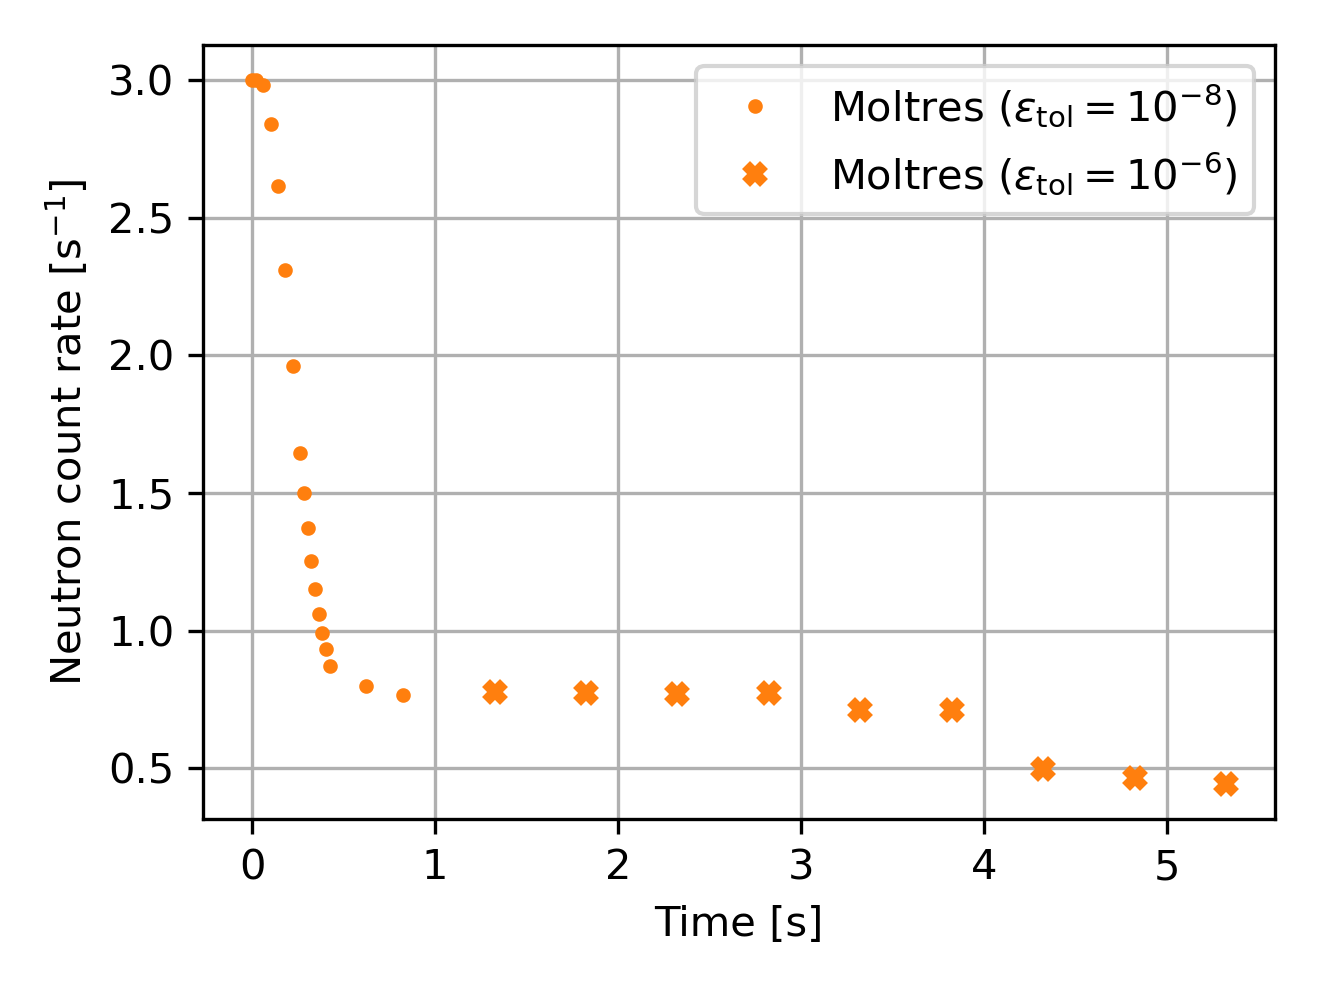
\includegraphics[width=0.78\columnwidth]{count-rate}
  \caption{Neutron count rate during the rod drop experiment from Moltres. The convergence tolerance
  of the neutron diffusion subsolver and the fixed point iterations was raised from $\epsilon=10^{-8}$
  to $10^{-7}$ from $t=1.32$ s onwards.}
  \label{fig:count-rate}
  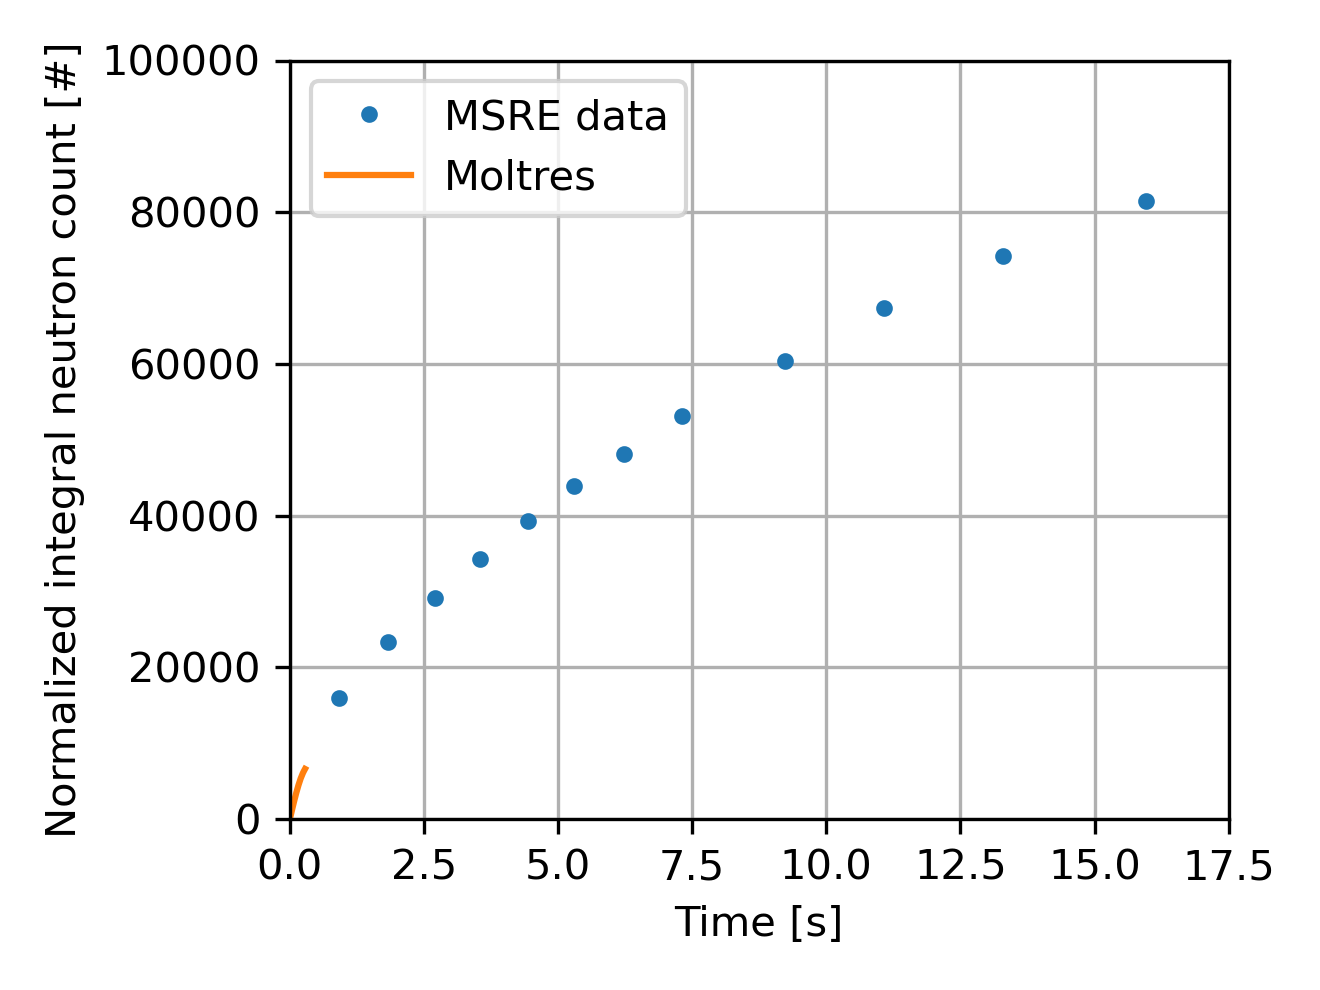
\includegraphics[width=0.78\columnwidth]{integral-count}
  \caption{Integral neutron count during the rod drop experiment from \gls{MSRE} experimental data
  and Moltres.}
  \label{fig:integral-count}
\end{figure}

\begin{figure}[p]
  \centering
  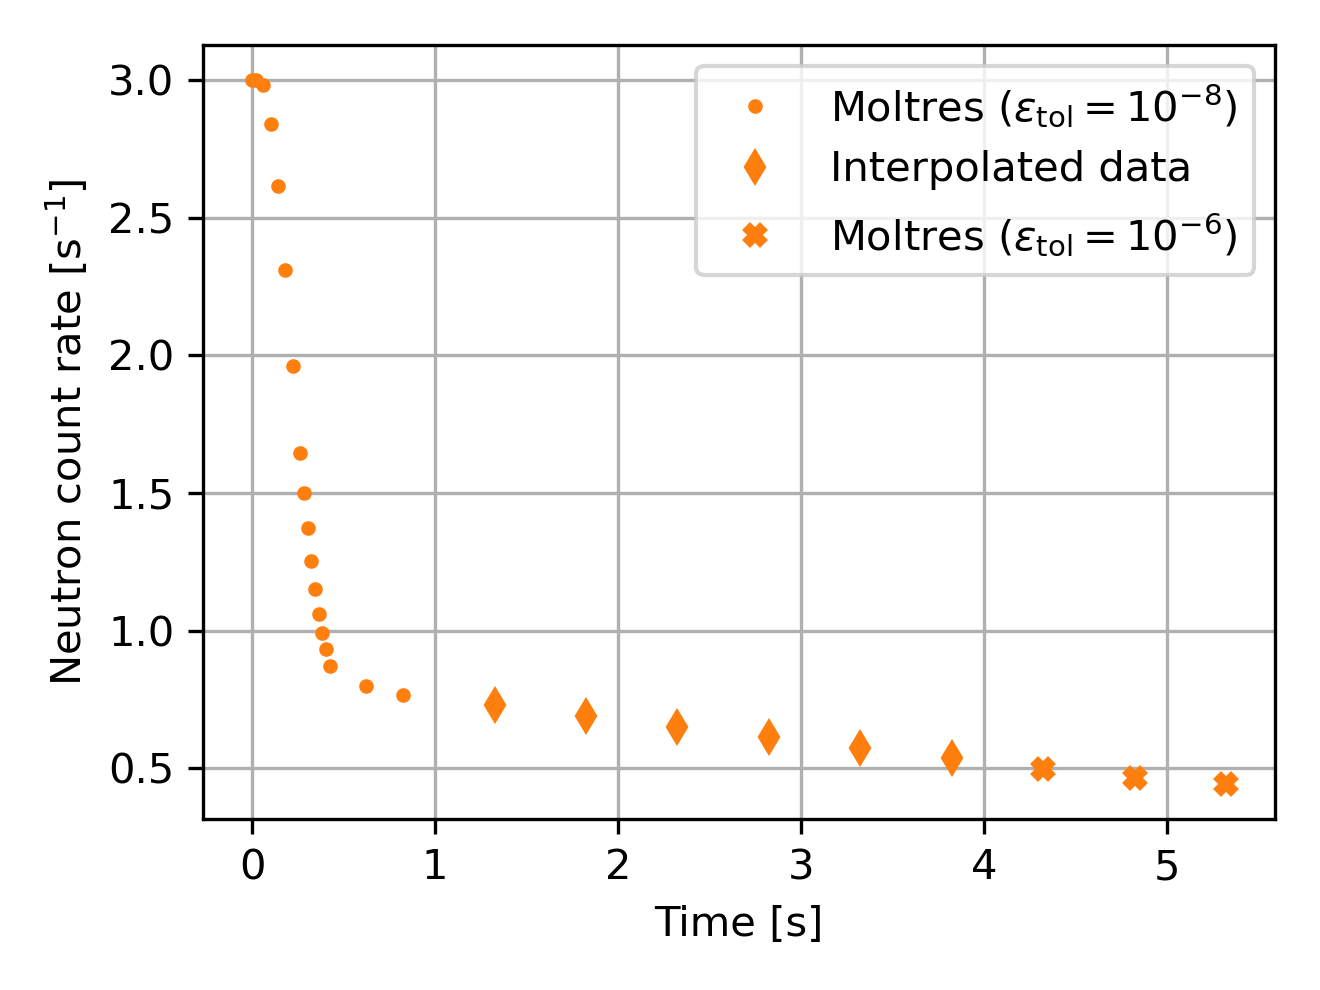
\includegraphics[width=0.78\columnwidth]{count-rate-interp}
  \caption{Neutron count rate during the rod drop experiment from Moltres with linearly interpolated
    data between $t=1.325$ s and $3.825$ s.}
  \label{fig:count-rate-interp}
  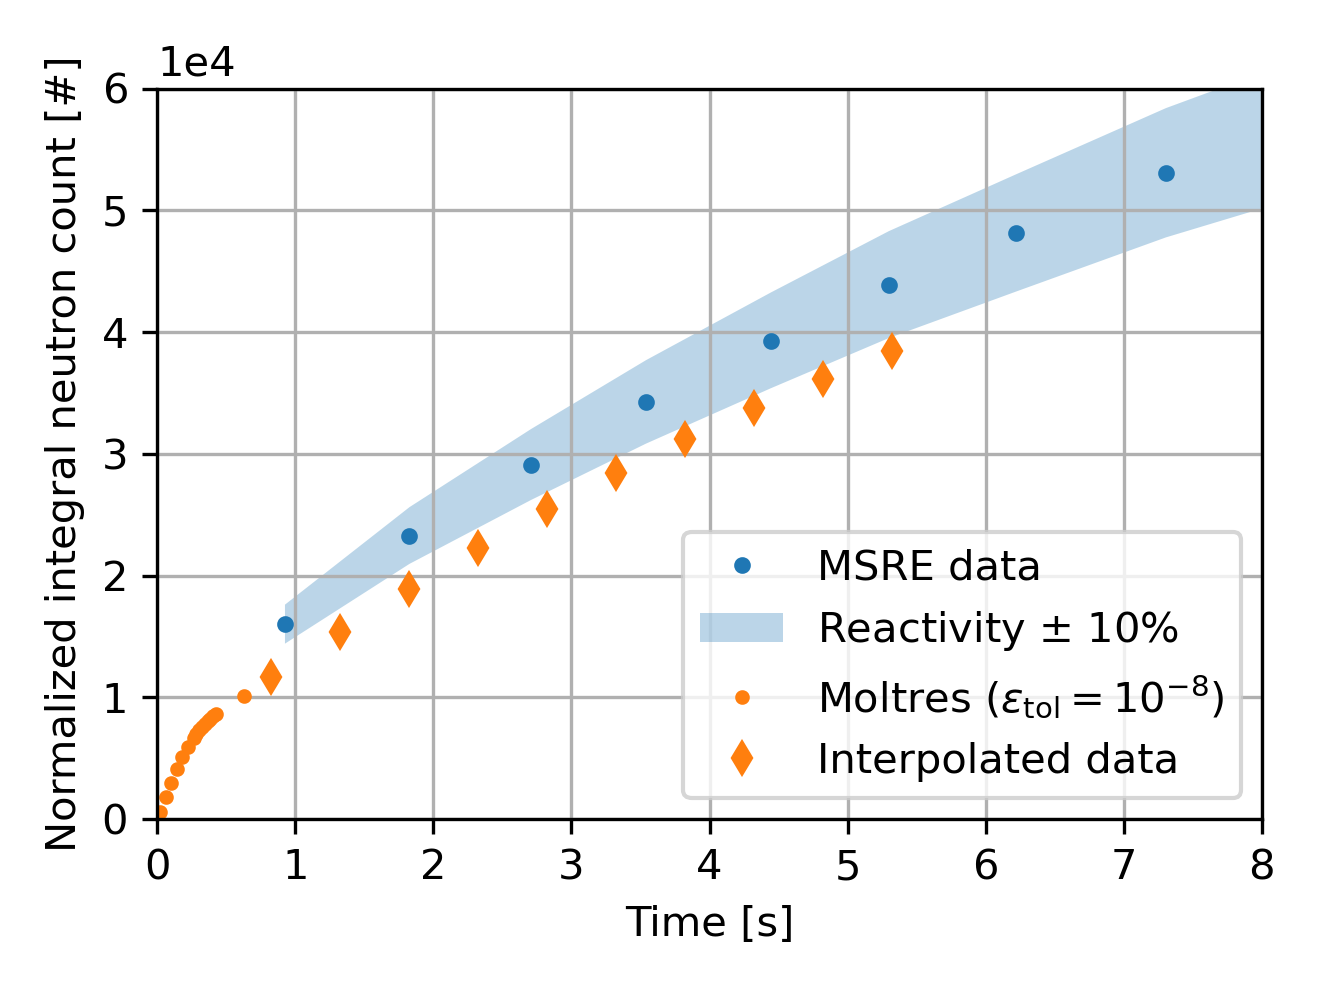
\includegraphics[width=0.78\columnwidth]{integral-count-interp}
  \caption{Integral neutron count during the rod drop experiment from \gls{MSRE} experimental data
  and Moltres with linearly interpolated count rate data between $t=1.325$ s and $3.825$ s.}
  \label{fig:integral-count-interp}
\end{figure}

Lagging solution states during the first fixed point iteration in each time-step also slowed
solution convergence, particularly when the control rod was in motion. This limited the simulation
from taking larger time-steps. Further work could include rearranging the nested coupling structure
or implementing relaxation schemes to improve solver numerical stability and convergence.

%Figures * show snapshots of the neutron group flux distributions at various times during the rod
%drop simulation. The neutron flux magnitudes fall as the reactor enters a sub-critical state. The
%Rod 1 induces a significant drop in neutron fluxes near the center of the core.

%\section{Reactivity Insertion Experiment} \label{sec:reactivity-insertion}
%
%After a long operational run on $^{235}$U fuel, \gls{ORNL} extended the \gls{MSRE} program to
%demonstrate reactor operation with $^{233}$U fuel. The \gls{MSRE} then became the first nuclear
%reactor to run on $^{233}$U bred from $^{232}$Th. During a series of tests for experimental
%dynamic analyses, \gls{MSRE} researchers conducted reactivity insertion tests with the reactor
%operating at 1, 5, and 8 MW \cite{steffy_experimental_1970}.
%In contrast to the rod drop experiments, these reactivity insertion
%experiments were conducted with the \gls{MSRE} in power operation.
%
%This work aims to replicate the power response following a reactivity insertion of 24.8 pcm of the
%\gls{MSRE} initially at 1 MW. Figure \ref{fig:msre-reactivity-insertion} shows the theoretical and
%experimental power response following the reactivity insertion. Three separate publications
%\cite{zanetti_innovative_2015, singh_study_2019, mochizuki_validation_2022} noted that the plot is
%mislabeled with the wrong reactivity insertion value of 0.0139 \% $\delta k/k$, which had been the
%reactivity insertion value for the 8 MW case. The correct reactivity insertion value is 24.8 pcm as
%mentioned prior.
%
%\begin{figure}[t]
%  \centering
%  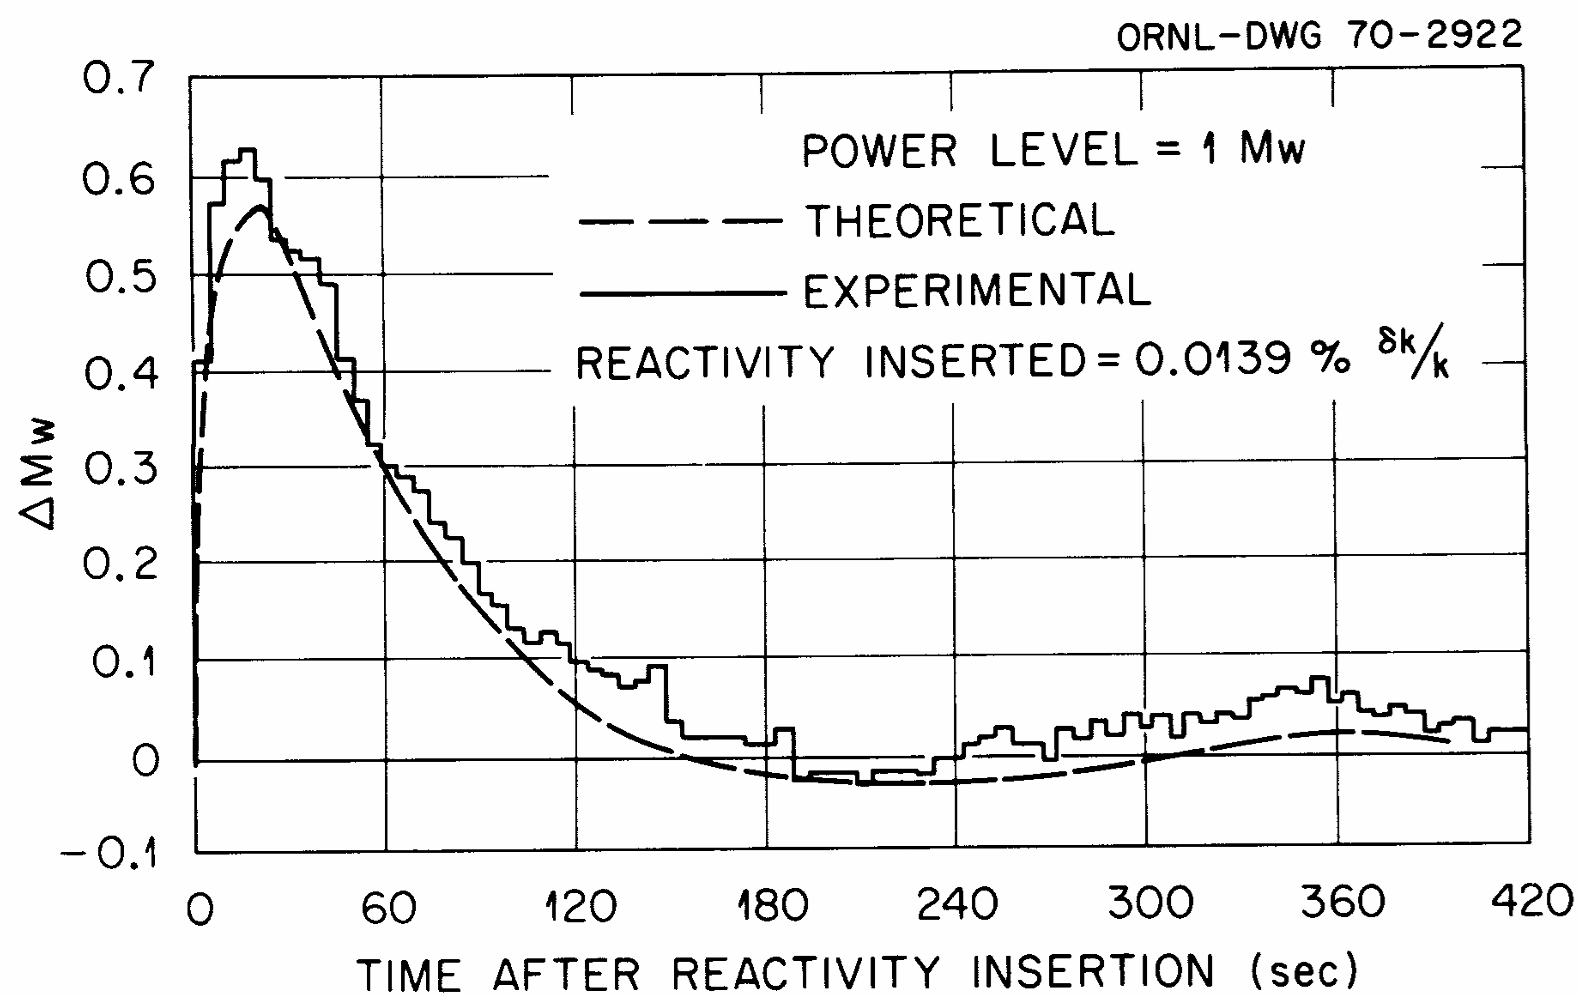
\includegraphics[width=0.8\columnwidth]{msre-reactivity-insertion}
%  \caption{Power response following a step reactivity insertion of 24.8 pcm with the reactor
%    initially at 1 MW \cite{steffy_experimental_1970}. Note that the authors of the \gls{MSRE}
%    report mislabeled the reactivity insertion value on the plot
%  \cite{zanetti_innovative_2015, singh_study_2019, mochizuki_validation_2022}.}
%  \label{fig:msre-reactivity-insertion}
%\end{figure}
%
%\subsection{Model Setup}
%
%For the reactivity insertion simulation, we must first identify the $^{233}$U salt composition used
%in the experiment. Power operations with the $^{233}$U-fueled \gls{MSRE} core
%occurred during Runs 16 to 18 according
%to \gls{MSRE} reports \cite{thoma_chemical_1971, burke_analysis_2019}. Table \ref{table:u233-salt}
%lists the proportion of elements in the \gls{MSRE} fuel salt during Runs 16 to 18. Note that the
%components do not sum up to 100 \% due to experimental uncertainty in chemical analysis and the
%presence of other elements that were not measured. Taking the nominal uranium value to be true, I scaled
%up the compositions of non-uranium elements to make up the remaining $(100\%-0.8155\%)$ of the salt. I
%kept the nominal weight percentage of uranium constant because it is the most accurate value in the table
%and has the biggest impact on the reactivity.
%%
%\begin{table}[t]
%  \small
%  \centering
%  \setlength\tabcolsep{4pt}
%  \caption{\gls{MSRE} fuel salt mean composition during the power operations with $^{233}$U \cite{thoma_chemical_1971}.
%  All values were measured via chemical analysis except the nominal U weight percentage, which was
%  calculated from inventory tracking of cumulative U additions to the salt.}
%  \begin{tabular}{l S[table-format=2.2(2)] S[table-format=1.2(2)] S[table-format=2.2(2)] S[table-format=2.2(3)] S[table-format=1.3(2)] S}
%    \toprule
%    Element & {Li} & {Be} & {Zr} & {F} & {U} & {U (Nominal)} \\
%    \midrule
%    Weight percentage [\%]  & 11.33(39) & 6.71(30) & 10.99(29) & 68.71(126) & 0.809(11) & 0.8155 \\
%    \bottomrule
%  \end{tabular}
%  \begin{tabular}{l S[table-format=2(1)] S[table-format=3(2)] S[table-format=2(2)] S}
%    \toprule
%    Element & {Cr} & {Fe} & {Ni} & {O} \\
%    \midrule
%    Parts per million [ppm] & 72(9) & 135(24) & 46(12) & 61 \\
%    \bottomrule
%  \end{tabular}
%  \label{table:u233-salt}
%\end{table}
%
%For the isotopic content of uranium, I used a composition restruction strategy developed by Burke
%\cite{burke_analysis_2019}. Their analysis determined that the $^{233}$U salt consists of residual
%salt from $^{235}$U operations, a depleted uranium feed, and a stock $^{233}$U feed. The residue
%and depleted uranium feed masses, taken from Burke's work, are 1.935 kg and 0.890 kg, respectively.
%The stock feed uranium
%mass is estimated to be 35.234 kg reported on January 12 1969 \cite{thoma_chemical_1971}. The
%experiment was performed on January 16 1969 \cite{steffy_experimental_1970}. Table 
%\ref{table:u233-composition} shows
%the breakdown and total isotopic content of uranium in the salt. The density of $^{233}$U salt is
%2.264 g cm$^{-3}$ at 911 K \cite{thoma_chemical_1971}.
%%
%\begin{table}[t]
%  \small
%  \centering
%  \setlength\tabcolsep{4pt}
%  \caption{Uranium isotopic composition reconstruction table \cite{burke_analysis_2019}.}
%  \begin{tabular}{l S S S S S S S}
%    \toprule
%    \multirow{2}{*}{Uranium Source} & {\multirow{2}{*}{Mass [kg]}} & \multicolumn{6}{c}{Weight percentage [\%]} \\
%                                    & & {$^{232}$U} & {$^{233}$U} & {$^{234}$U} & {$^{235}$U} & {$^{236}$U} & {$^{238}$U} \\
%                                    \cmidrule(r){1-1} \cmidrule(rl){2-2} \cmidrule(l){3-8}
%    Residue & 1.935 & & & 0.343 & 32.705 & 0.483 & 66.469 \\
%    Depleted & 0.890 & & & & 0.3 & & 99.7 \\
%    Stock & 35.234 & 0.02 & 91.49 & 7.6 & 0.7 & 0.05 & 0.14 \\
%    \bottomrule
%  \end{tabular}
%  \label{table:u233-composition}
%\end{table}
%
%Due to constraints on computational resources, the reactivity insertion simulation ran a 3-D
%quarter-core \gls{MSRE} model. Refer to Figure \ref{fig:1/4-geom} for the horizontal cross section
%view of the 3-D quarter-core model. Figure * shows the side view from a vertical side of the
%quarter-core and the direction of salt flow in each major region. The regions are the salt-graphite
%lattice, the upper plenum, the out-of-core components, the downcomer, and the lower plenum. The
%model assumes a flat salt velocity profile in each region. The actual total volumetric flow rate of
%the \gls{MSRE} is 1200 gpm (gallons per minute) \cite{robertson_msre_1965}. Dividing this value by
%four for the quarter-core model and converting to SI units gives a volumetric flow rate of
%0.01893 m$^3$ s$^{-1}$.
%
%Table \ref{table:msre-flow} lists the dimensions, salt flow velocities, and salt residence
%times in each region to maintain the calculated volumetric flow rate. The salt residence times are
%consistent with \gls{MSRE} specifications \cite{robertson_msre_1965}. The out-of-core region is
%modeled as a 1-D pipe due to its lower neutronic importance other than \gls{DNP} decay and heat
%removal through the heat exchanger. The out-of-core region salt velocity is set to the same magnitude
%as the downcomer for ease of implementation with the height adjusted accordingly to maintain the
%out-of-core salt residence time. Note that the velocity in the downcomer is negative since salt
%flows downwards unlike in the other regions.
%%
%\begin{table}[t]
%  \small
%  \centering
%  \caption{Dimensions, salt flow velocities, and salt residence times in each region of the \gls{MSRE}.}
%  \begin{tabular}{l S S S S}
%    \toprule
%    Component & {Salt cross-sectional area [m$^2$]} & {Height [m]} & {Velocity [m s$^{-1}$]} & {Time [s]} \\
%    \cmidrule(r){1-1} \cmidrule(l){2-5}
%    Upper plenum & 0.42411 & 0.2539 & 0.04463 & 5.69 \\
%    Lattice      & 0.08646 & 1.6637 & 0.21891 & 7.60 \\
%    Lower plenum & 0.42614 & 0.1875 & 0.04935 & 3.80 \\
%    Out-of-core  & {-}     & 5.3081 & 0.65532 & 8.1 \\
%    Downcomer    & 0.02888 & 1.6637 & -0.65532 & 2.539 \\
%    \bottomrule
%  \end{tabular}
%  \label{table:msre-flow}
%\end{table}
%
%% Unlike with $^{235}$U salt, there is no widely recognized benchmark value
%% for the density of $^{233}$U salt. During \gls{MSRE} operation, researchers were still developing
%% reliable techniques for measuring the density of molten salt mixtures \cite{thoma_chemical_1971}.
%% \gls{MSRE} $^{233}$U fuel salt with has a lower density than $^{235}$U salt largely due to its
%% lower $^{238}$U content. 
%
%The MultiApp nested iterative coupling structure for this reactivity insertion simulation is similar
%to the implementation for the rod drop simulation. Figure \ref{fig:insertion-coupling}
%provides an updated illustration of the nexted iteration coupling with temperature. The \gls{DNP}
%and temperature distributions are solved together with additive Schwarz method preconditioning in
%Moltres since they are both advective problems. The 1-D out-of-core model accounts for \gls{DNP}
%loss and heat removal outside the core. Delayed neutrons produced in this region are considered
%lost and do not contribute to the neutron flux in the core.
%
%\begin{figure}[t]
%  \tikzstyle{every node}=[font=\small]
%  \centering
%  \begin{tikzpicture}
%    \node (1) [solver] {\textbf{$\bm{S_N}$ transport subsolver}};
%    \node (2) [solver, right of=1, xshift=4cm] {\textbf{Neutron\\ diffusion\\ subsolver}};
%    \node (3) [solver, right of=2, xshift=4cm] {\textbf{In-core DNP \& temperature subsolver}};
%    \node (4) [solver, below of=3, yshift=-3cm] {\textbf{Ex-core DNP \& temperature subsolver}};
%    \draw [arrow] (1.10) -- node[anchor=south, text width=4cm, align=center] {$\vec{D}_g, \gamma_g$} (2.170);
%    \draw [arrow] (2.190) -- node[anchor=north, text width=4cm, align=center] {$\phi_g, C_i, T$} (1.350);
%    \draw [arrow] (2.10) -- node[anchor=south, text width=4cm, align=center] {$Q_f, Q$} (3.170);
%    \draw [arrow] (3.190) -- node[anchor=north, text width=4cm, align=center] {$C_i, T$} (2.350);
%    \draw [arrow] (3.280) -- node[anchor=west, text width=1cm, align=center] {$C^\text{out}_i$\\ $T^\text{out}$} (4.80);
%    \draw [arrow] (4.100) -- node[anchor=east, text width=1cm, align=center] {$C^\text{in}_i$\\ $T^\text{in}$} (3.260);
%    \node (5) [bound, fit=(3) (4), label={[align=center,rotate=90]left:\textbf{Salt loop}\\}] {};
%    \node (6) [bound, fit=(2) (5), label={[align=center,rotate=90]left:\textbf{Inner iteration}\\}] {};
%    \node (7) [bound, fit=(1) (6), label={[align=center,rotate=90]left:\textbf{Outer iteration}\\}] {};
%  \end{tikzpicture}
%  \caption{The nested iteration structure coupling the $S_N$, neutron diffusion,
%  in-core \gls{DNP}-temperature, and ex-core
%  solvers for the reactivity insertion simulation using the hybrid $S_N$-diffusion method.}
%  \label{fig:insertion-coupling}
%\end{figure}
%
%The reactivity insertion simulation requires a prior ``steady-state'' simulation to obtain the group
%flux, \gls{DNP}, and temperature distributions under 1 MW power operation and steady salt flow. The
%``steady-state'' simulation is a time-dependent simulation with timestep sizes of 1 s to advance
%the model towards 1 MW steady state operation. Following this, the reactivity insertion simulation
%uses the \gls{MOOSE} Restart capability to load in variable distributions for the initial conditions.
%
%\subsection{Preliminary Rod Worth Calculations}
%
%The control rod worth of the \gls{MSRE} quarter-core model with $^{233}$U fuel must be determined
%to estimate the initial rod height and rod travel necessary for the reactivity insertion
%simulation. We start this process with comparisons of Rod 1 worths between a full-core OpenMC model
%and experimental data. Table \ref{table:u233-rod-worth} compares the total rod worth of Rod 1 at
%922 K between the OpenMC model from this work
%and \gls{MSRE} data. The rod worth estimate from OpenMC agrees closely with the predicted (i.e.,
%calculated) \gls{MSRE} value. The measured \gls{MSRE} rod worth value is about 7 \% smaller than
%the predicted value. \gls{MSRE} researchers noted poor precision in their rod worth measurements
%due to ``wear and aging'' in the control rod drive assembly \cite{engel_zero-power_1972}. This may
%be responsible for some uncertainty. However, the actual rod worth is likely closer to the measured
%value than the predicted value, and the \gls{MSRE} model of this work is likely to contain as yet
%unknown biases. Nevertheless, the rod worth estimate is close enough that it should not affect the
%\gls{MSRE} power response following a fixed reactivity insertion.
%%
%\begin{table}[t]
%  \centering
%  \caption{Total rod worth of Rod 1 at 922 K from OpenMC full-core \gls{MSRE} model and \gls{MSRE}
%  experimental data.}
%  \begin{tabular}{l S[table-format=4(3)] S}
%    \toprule
%    & {Rod worth [pcm]} & {Percentage discrepancy [\%]} \\
%    \cmidrule(r){1-1} \cmidrule(l){2-3}
%    MSRE (measured) & 2580(129) & {-} \\
%    MSRE (predicted) & 2750 & 6.6 \\
%    OpenMC (this work) & 2771 & 7.4\\
%    \bottomrule
%  \end{tabular}
%  \label{table:u233-rod-worth}
%\end{table}
%
%The 3-D quarter-core \gls{MSRE} model for the reactivity insertion simulation contains only one
%control rod, but it is equivalent to four rods due to rotational symmetry of the quarter-core model.
%The total rod worth of the 3-D quarter-core \gls{MSRE} model using the hybrid method on Moltres is
%9702 pcm, just under four times the worth of Rod 1 from Table \ref{table:u233-rod-worth} due to
%rod shadowing effects that reduce the worth of adjacent control rods. Figure \ref{fig:u233-rod-worth-curve} shows the rod
%worth values from Moltres for the 3-D quarter-core model and the monotone cubic spline interpolation
%curve. Despite having fewer data points than the $^{235}$U rod worth analysis (Section
%\ref{sec:3d-nts}), this interpolation curve is valid for the reactivity insertion experiment since
%the rod heights will strictly remain within the middle
%range where the change in rod worth is approximately linear to changes in rod height.
%
%The required
%rod travel in the quarter-core model for a 24.8 pcm reactivity insertion in this linear region
%is 0.105 inches (0.267 cm). The estimated rod travel required to induce the same reactivity
%insertion in the actual \gls{MSRE} reactor is 0.396 inches (1.00 cm) obtained by scaling with the
%total measured \gls{MSRE} rod worth in Table \ref{table:u233-rod-worth}. Using
%an estimated rod speed of 1.27 cm s$^{-1}$ \cite{robertson_msre_1965}, the reactivity insertion
%occurs over a 0.791-s ramp (reactivity insertions at this timescale are considered step reactivity
%insertions). The rod is assumed to accelerate and decelerate instantaneously given
%the low rod speed.
%The reactivity insertion simulation ran with timestep sizes of 0.198 s during rod movement and
%0.25 s after the rod reaches its final position. These timestep sizes were chosen based on
%considerations balancing accuracy and available computational resources. The main purpose of this
%work is the demonstration of the hybrid method for time-dependent control rod modeling; a detailed
%time-stepping truncation error analysis is out of the scope of this work.
%
%\begin{figure}[t]
%  \centering
%  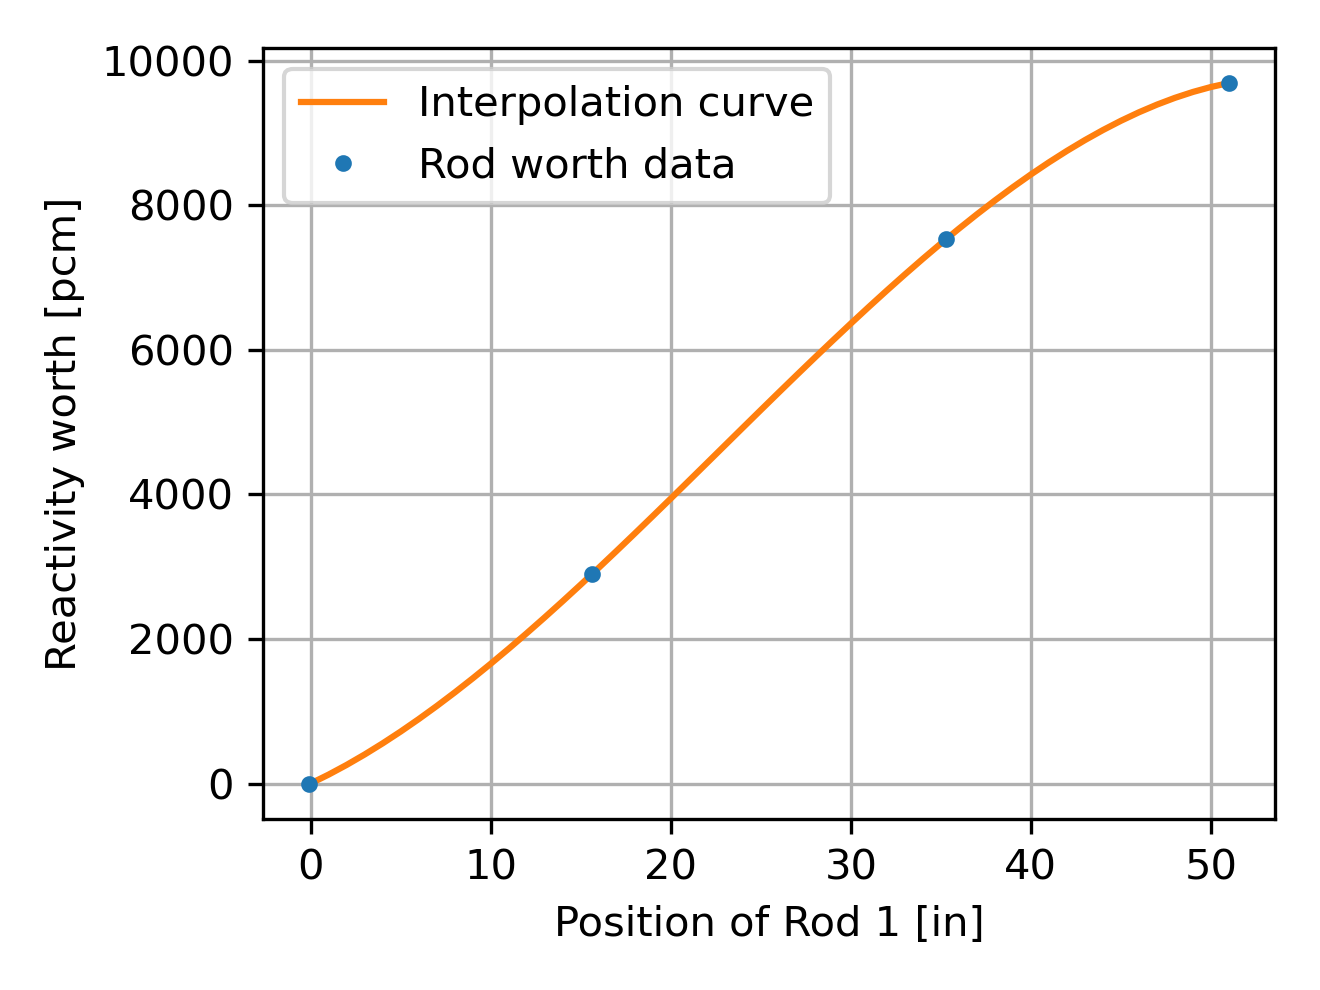
\includegraphics[width=0.8\columnwidth]{u233-rod-worth-curve}
%  \caption{Rod worth data points and the monotone cubic spline interpolation curve from $k$-eigenvalue
%  hybrid method simulations on the 3-D quarter-core \gls{MSRE} model.}
%  \label{fig:u233-rod-worth-curve}
%\end{figure}
%
%\subsection{Temperature Reactivity Coefficient}
%
%This work compares isothermal temperature reactivity coefficients calculated from $k_\text{eff}$
%values measured at 872 K and 972 K with the $^{233}$-fueled \gls{MSRE} at operating fuel
%concentration. This approach is identical to that
%of the \gls{MSRE} experimental measurements \cite{engel_zero-power_1972} and the temperature
%coefficient calculation procedure used for the $^{235}$U-fueled \gls{MSRE} in Section
%\ref{sec:temp-coef}.
%
%Table \ref{table:temp-coef-u233} compares the isothermal reactivity coefficients from the experimental
%and numerical sources. No uncertainty data is available from the relevant \gls{ORNL} report
%\cite{engel_zero-power_1972}. However, the authors noted significantly different readings ranging
%from 12.4 to 15.3 pcm K$^{-1}$ due to gas bubbles introduced by the salt pump. The
%presence of gas bubbles led to smaller reactivity coefficient measurements. The numerical OpenMC
%and hybrid models overestimate the temperature reactivity coefficient magnitude by 12 \% and 11 \%,
%respectively, relative to the experimental data.
%
%\begin{table}[t]
%  \small
%  \centering
%  \caption{Isothermal temperature reactivity coefficients with $^{233}$U-fueled \gls{MSRE} from
%    \gls{MSRE} experimental data, \gls{MSRE} predicted value, and the OpenMC
%  and Moltres models in this work.}
%  \begin{tabular}{l S[separate-uncertainty=true,table-format=2.2(2)] S}
%    \toprule
%     & {Temperature coefficient [pcm K$^{-1}$]} & {Percentage discrepancy [\%]}\\
%     \cmidrule(rl){2-2} \cmidrule(l){3-3}
%    \gls{MSRE} experimental data & -15.3 & {-}\\
%    \gls{MSRE} predicted value & -15.8 & -3.4 \\
%    OpenMC (This work) & -17.14 & -12 \\
%    Hybrid (This work) & -16.96 & -11 \\
%    \bottomrule
%  \end{tabular}
%  \label{table:temp-coef-u233}
%\end{table}
%
%\subsection{Reactivity Insertion Numerical Results \& Discussion}
%
%Figure \ref{fig:insertion-power} shows the \gls{MSRE} data and simulation results for change in
%power output following the 24.8 pcm reactivity
%insertion. From the experimental data, the power output rises rapidly at the start of the
%reactivity insertion before oscillating back down below the initial power output. Power output
%peaks again later at around $t=360$ s. Moltres reproduces the same trend in power output, but 
%over/under-predicts the first power peak by y \%. It also over/under-predicts the subsequent power
%oscillations.
%Significant contributors to the discrepancies are the uncertainties in the physical properties of
%the fuel salt, temperature reactivity coefficient, and the dynamic response of the heat exchanger.
%
%Figure \ref{fig:insertion-temperature} shows the maximum fuel salt and graphite temperatures, and
%the mean salt inlet and outlet
%temperatures following the reactivity insertion. The increase in maximum temperatures is more
%gradual than the increase in power output as the salt and graphite take time to heat up. The salt
%outlet temperature follows closely behind as the heated salt flows out of the core. The salt inlet
%temperature lags behind the other temperature measurements due to the time taken for the heated
%salt to travel through the out-of-core region. The temperature values appear to settle at higher
%temperatures to compensate for the inserted reactivity.
%
%\begin{figure}[t]
%  \centering
%%  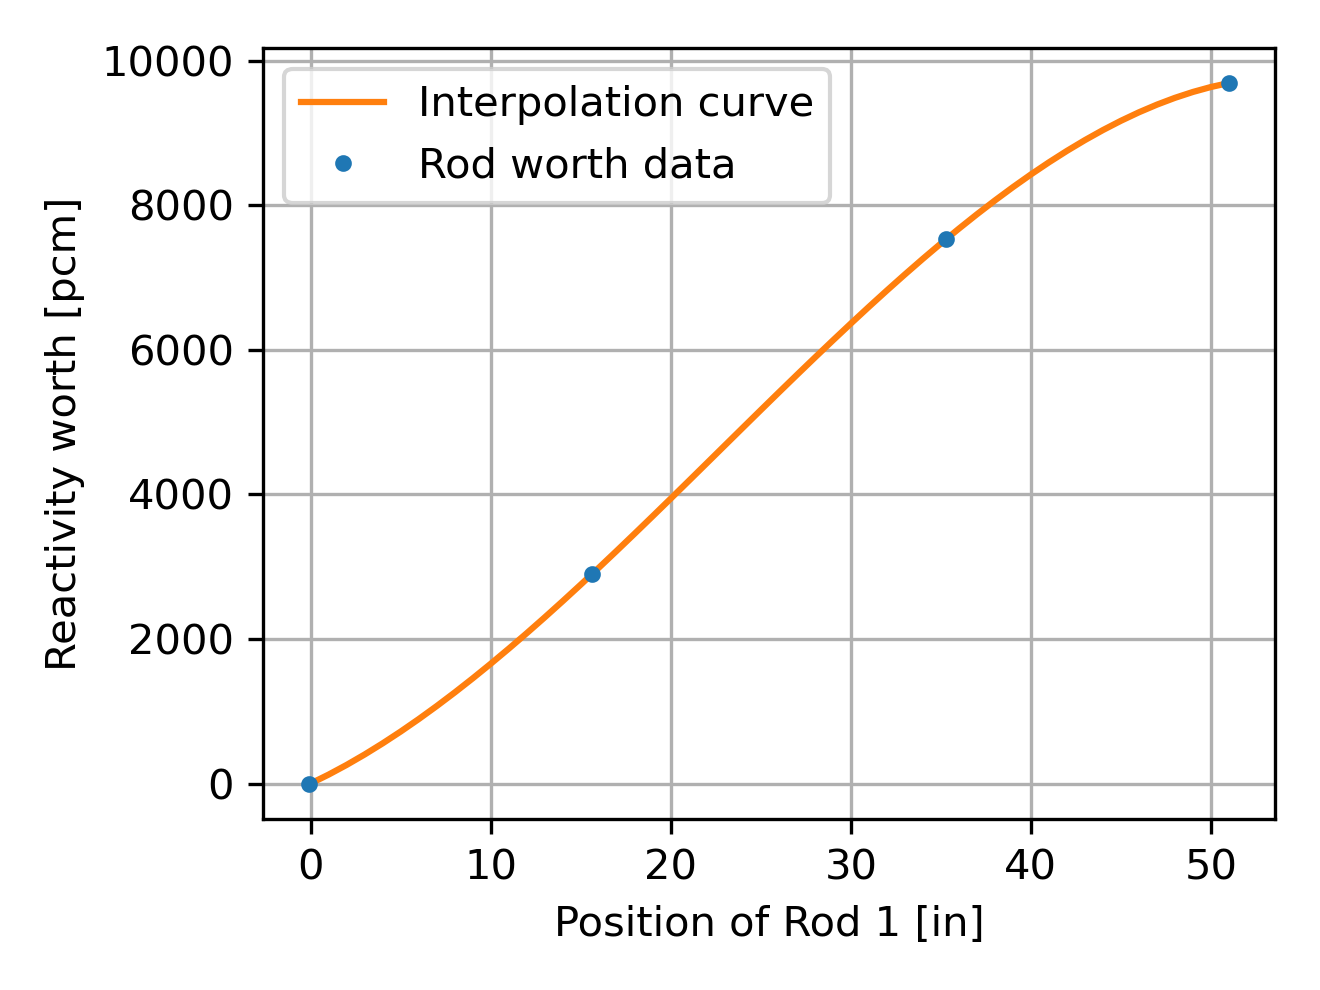
\includegraphics[width=0.8\columnwidth]{u233-rod-worth-curve}
%  \caption{Change in power output following a step reactivity insertion of 24.8 pcm with the
%  \gls{MSRE} initially at 1 MW.}
%  \label{fig:insertion-power}
%\end{figure}
%
%\begin{figure}[t]
%  \centering
%%  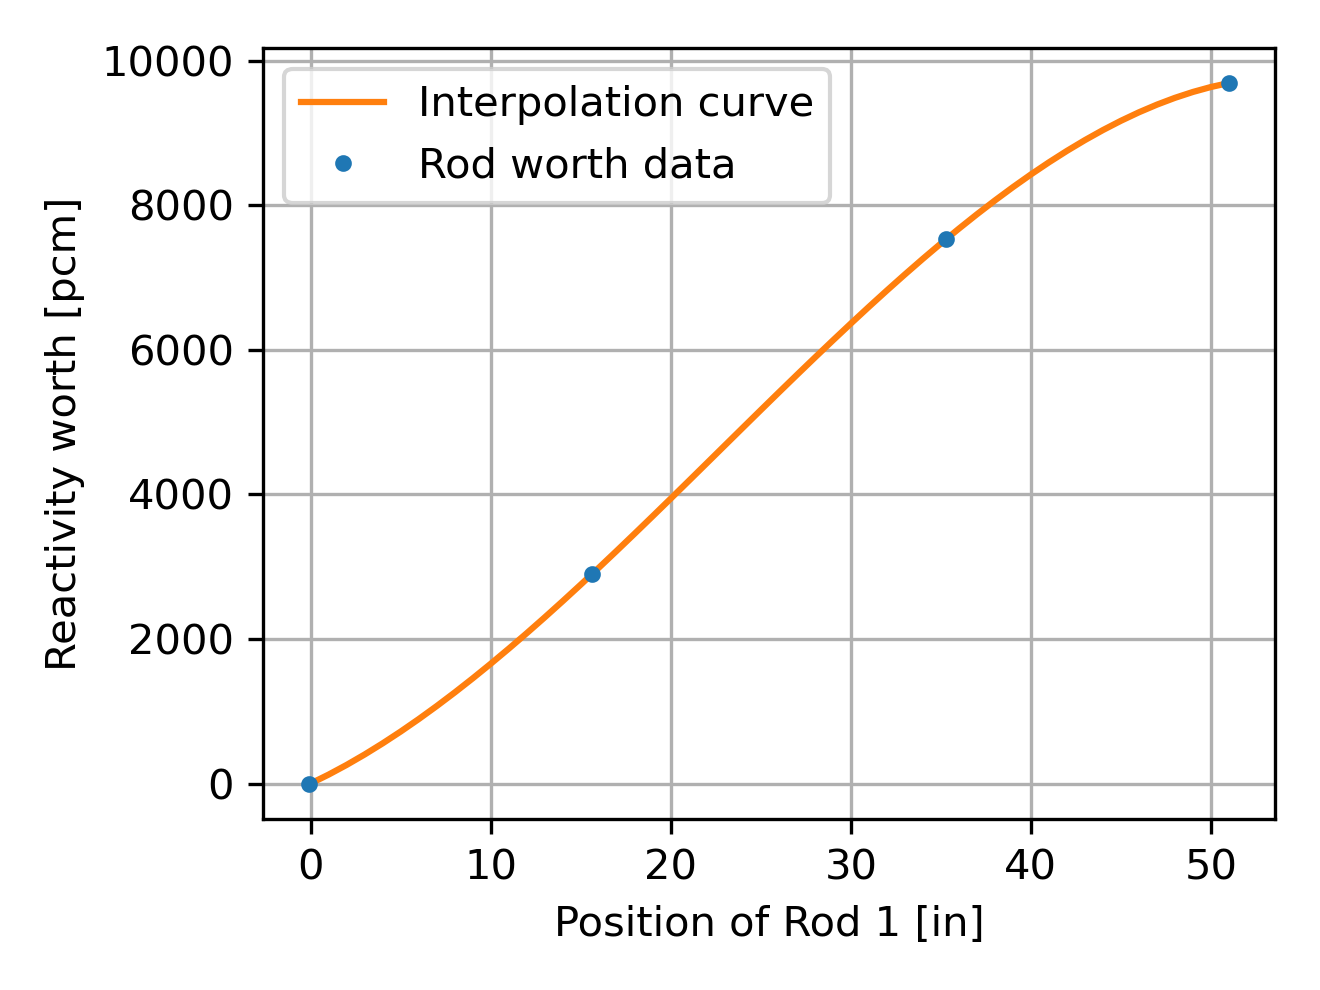
\includegraphics[width=0.8\columnwidth]{u233-rod-worth-curve}
%  \caption{Change in maximum fuel salt and graphite temperatures, and the mean salt inlet and outlet
%  temperatures following a step reactivity insertion of 24.8 pcm with the \gls{MSRE} initially at 1
%  MW.}
%  \label{fig:insertion-temperature}
%\end{figure}

\FloatBarrier

\section{Summary} \label{sec:transient-summary}

%The hybrid $S_N$-diffusion method combines the strengths of the $S_N$ and neutron
%diffusion methods accurately model control rods while remaining tractable on modest computational
%resources. This chapter covers work demonstrating the hybrid $S_N$-diffusion method through two
%time-dependent reactivity-initiated simulations. The hybrid $S_N$-diffusion solver implemented in
%Moltres is coupled to preexisting \gls{DNP} and temperature solver capabilities to model
%transient behavior in reactors. 
%
%The first time-dependent simulation is based on a zero-power \gls{MSRE} rod drop experiment. The
%rod drop is estimated to induce a 1500 pcm reactivity withdrawal in the \gls{MSRE}. Preliminary
%calculations determined the required initial rod height in the numerical model to replicate the
%same reactivity withdrawal effect and eliminate rod worth discrepancies. Following an initial
%$k$-eigenvalue simulation to obtain initial flux and \gls{DNP} distributions, the rod drop
%simulation ran with total fission neutron production rate measurements at each timestep. The
%integral neutron production, normalized to match the initial experimental neutron count rate,
%showed good agreement with the experimental integral neutron count curve following the rod drop.
%The numerical result has a maximum discrepancy of x \% at $t=16$ s. Experimental uncertainties in
%the actual $^{235}$U content, initial rod height, rod acceleration, and the initial neutron count
%rate may be responsible for some of the discrepancy. Snapshots of the 3-D neutron group flux
%distributions at various timesteps show expected localized flux decreases around the control rod
%as it moves through the core.
%
%The second time-dependent simulation is based on a reactivity insertion experiment on the
%$^{233}$U-fueled \gls{MSRE}. A control rod withdrawal induces a 24.8 pcm step reactivity
%insertion on the \gls{MSRE} initially running at 1 MW with steady salt flow. Moltres reproduces
%the general shape of the first power peak and the subsequent power oscillations. The power peak
%magnitude differs by y \% compared to \gls{MSRE} data. The fuel
%salt, graphite, inlet, and outlet temperature measurements show delayed responses to the increase
%in power output due to the time taken for the salt and graphite to heat up. The temperature values
%eventually settle higher than the initial
%state to compensate for the reactivity insertion.
%
%Overall, this work has successfully demonstrated the hybrid method for coupled time-dependent
%reactor analyses of reactivity-initiated transients involving control rods.

The hybrid $S_N$-diffusion method combines the strengths of the $S_N$ and neutron
diffusion methods to accurately model control rods while remaining tractable on modest computational
resources. This chapter covers work demonstrating the hybrid $S_N$-diffusion method through a
time-dependent reactivity-initiated simulation. The hybrid $S_N$-diffusion solver implemented in
Moltres is coupled to preexisting \gls{DNP} and temperature solver capabilities to model
transient behavior in reactors.

The time-dependent simulation is based on a zero-power \gls{MSRE} rod drop experiment. The
rod drop is estimated to induce a 1500 pcm reactivity withdrawal in the \gls{MSRE}. Preliminary
calculations determined the required initial rod height in the numerical model to replicate the
same reactivity withdrawal effect and eliminate rod worth discrepancies. Following an initial
$k$-eigenvalue simulation to obtain initial flux and \gls{DNP} distributions, the rod drop
simulation ran with total fission neutron production rate measurements at each timestep. The
integral neutron production, normalized to match the initial experimental neutron count rate,
showed good agreement with the experimental integral neutron count curve following the rod drop.
Convergence issues with the nested coupling structure of the hybrid method and the \gls{DNP}
subsolver impacted the precision of several data points during the simulation.
Future investigations could look into alternative nested solver coupling structures and relaxation
schemes to resolve these issues.
Experimental uncertainties in the actual $^{235}$U concentration, initial \& final rod heights, rod
acceleration, and the initial neutron count rate were also responsible for discrepancies relative
to experimental data.
%Snapshots of the 3-D neutron group flux
%distributions at various timesteps show expected localized flux decreases around the control rod
%as it moves through the core.
Overall, this work has successfully demonstrated the hybrid method for coupled time-dependent
reactor analysis of reactivity-initiated transients involving control rods.
